\vspace{-0.5em}
\section{Results}
\label{sec:Result}
In this section, we report the experimental results of the HDP approach by
significance attribute selection for metric selection and KSAnalyzer with the cutoff threshold of 0.05.

Among different
metric selections, significance attribute selection led to the best
prediction performance overall. In terms of analyzers, KSAnalyzer led
to the best prediction performance.
Since the KSAnalyzer is based on the p-value of a statistical test, we chose
a cutoff of 0.05 which is a commonly accepted significance level in the
statistical test~\cite{Corder09}.

\vspace{-0.2em}
%----------------------------------------------------------
\subsection{Comparison Result with Baselines} % KSAnalyzer with the cutoff of %
% 0.05}
%----------------------------------------------------------

\begin{table}[!t]
%\footnotesize
%\small
\scriptsize
\centering
\caption{Comparison results among WPDP, CPDP-CM, CPDP-IFS,
and HDP by KSAnalyzer with the cutoff of 0.05 in a median AUC.
%  Outperforming results with statistical
%  significance (Wilcoxon signed-rank test, p$<$0.05) between within and cross by
%  the proposed approach and between cross using common features and those by the
%  proposed approach are bold-faced and underlined respectively.
}
\label{tab:result_overview}
%\setlength{\tabcolsep}{5pt}
%\setlength{\extrarowheight}{1.5pt}
\begin{tabular}{|@{ }c@{ }||@{ }c@{ }|@{ }c@{ }|@{ }c@{ }||@{ }c@{ }|}
%\begin{tabular}{|c||c|c|c||c|}
\hline
{\bf Target}
& \specialcell{{\bf WPDP}\\{(Baseline1)}} 
&\specialcell{{\bf CPDP-CM}\\{(Baseline2)}}
&\specialcell{{\bf CPDP-IFS}\\{(Baseline3)}}
&\specialcell{{\bf HDP}\\{\bf KSAnalyzer}\\{cutoff=0.05}}
\\
\hline \hline

EQ			&0.583	& 0.776	&0.461  &0.783		\\ \hline
JDT			&0.795	& 0.781 	&0.543	&0.767	 \\ \hline
LC			&0.575	& 0.636 &0.584	&0.655		\\ \hline
ML			&{\bf 0.734}	& 0.651 &0.557	&0.692*		\\ \hline
PDE			&0.684	& 0.682 &0.566	&0.717	 	\\ \hline \hline

Apache		&0.714	& 0.689  &0.635	&\underline{0.717}*		\\ \hline
Safe			&0.706	& 0.749  &0.616	&{\bf \underline{0.818}}*	 	\\ \hline
Zxing		&0.605	& 0.619  &0.530	&{\bf \underline{0.650}}*		\\ \hline \hline

ant-1.3		&0.609	& 0.590	&0.500	&0.835	 \\ \hline
arc			&0.670	& 0.611 &0.523	&0.701		\\ \hline
camel-1.0	&0.550	& 0.590	&0.500	&0.639	\\ \hline
poi-1.5		&0.707	& 0.676 &0.606	&0.701		\\ \hline
redaktor		&0.744	& 0.500 &0.500	&0.537		\\ \hline
skarbonka	&0.569	& 0.736 &0.528	&{\bf 0.694}*	 	\\ \hline
tomcat		&0.778	& 0.746 &0.640	&0.818		\\ \hline
velocity-1.4	& 0.725	& 0.609 &0.500	&0.391		\\ \hline
xalan-2.4	&0.755	& 0.658 &0.499	&0.751		\\ \hline
xerces-1.2	&0.624	& 0.453 &0.500	&0.489		\\ \hline \hline

cm1			&0.653	& 0.622 &0.551	&{\bf \underline{0.717}}*	 \\ \hline
mw1			&0.612	& 0.584 &0.614	& 0.727		\\ \hline
pc1			&0.787	& 0.675 &0.564	&0.752*		\\ \hline
pc3			&{\bf 0.794}	& 0.665 &0.500	&\underline{0.738}*		\\ \hline
pc4			&{\bf 0.900}	& 0.773 &0.589	&0.682*	 \\ \hline \hline

ar1		&0.582	& 0.464  &0.500	&{\bf \underline{0.734}}*		\\ \hline
ar3		&0.574	& 0.862 &0.682	&{\bf 0.823}*	 	\\ \hline
ar4		&0.657	& 0.588 &0.575	&{\bf \underline{0.816}}*	 \\ \hline
ar5		&0.804	& 0.875	&0.585	&0.911*	\\ \hline
ar6		&0.654	& 0.611 &0.527	&\underline{0.640}		\\ \hline \hline \hline

{\bf {\em All}} & 0.657 & 0.636 &0.555	& \underline{\bf 0.724}*  \\ \hline


\end{tabular}
\end{table}

% 
% \begin{figure*}[t]
% 	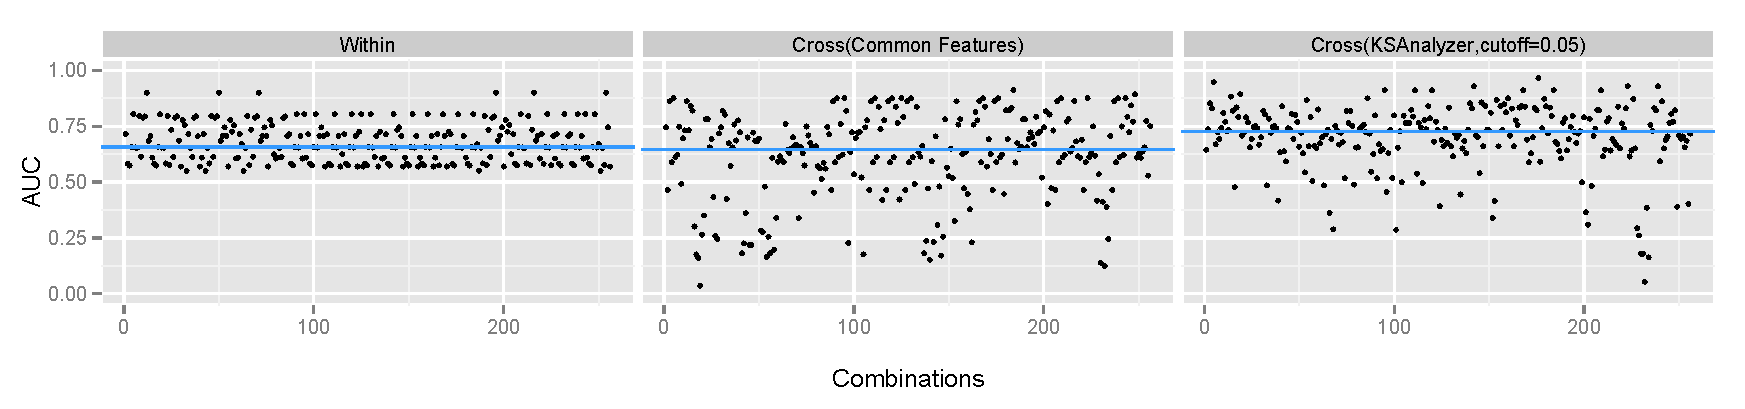
\includegraphics[width=\linewidth]{Figures/Result/auc_compare.pdf}
% 	\caption{Prediction performance variance among within-prediction,
% 	cross-prediction using common metrics, and cross-prediction by KSAnalyzer with
% 	the cutoff of 0.05 in terms of AUC. The number of prediction combinations is 256.}
% 	\label{fig:compare_results_on_defect}
% \end{figure*}


Table~\ref{tab:result_overview} shows the prediction performance (a median AUC)
of baselines and HDP by KSAnalyzer with the cutoff of 0.05,
for each target as well as all targets (the last row in the table). Baseline1 represents
the WPDP results of a target project and Baseline2 shows
the CPDP results using common metrics (CPDP-CM) between source and target
projects. Baseline3 shows the results of CPDP-IFS proposed by He et
al.~\cite{He14}. The last column shows the HDP results by KSAnalyzer with the
cutoff of 0.05. If there are better results between Baseline1 and our approach with statistical significance (Wilcoxon signed-rank
test~\cite{Wilcoxon45}, p$<$0.05), the better AUC values are in
bold font as shown in Table~\ref{tab:result_overview}.
Between Baseline2 and our approach, better AUC values with
statistical significance are underlined in
the table. Between Baseline3 and our approach, better AUC values with
statistical significance are shown with an asterisk (*).

%From Table~\ref{tab:result_overview}, 
We observed the following results about RQ1:
\squishlist
	\item In 25 out of 28 targets, HDP by KSAnalyzer with the cutoff of
	0.05 leads to better or comparable results against WPDP with statistical
	significance. (The WPDP results in only ML, pc3, and pc4 are in bold font.)
	\item HDP by KSAnalyzer with the cutoff of 0.05 outperforms
	WPDP with statistical significance when considering
	results from all targets ({\em All} in the last row in the table) together in
	our experimental settings.
\squishend  

The following results are related to RQ2:
\squishlist 	
	\item HDP by KSAnalyzer with the cutoff of 0.05
	leads to better or comparable results to CPDP-CM
	with statistical significance. (no underlines in CPDP-CM of
	Table~\ref{tab:result_overview})
	\item HDP by KSAnalyzer with the cutoff of 0.05 outperforms
	CPDP-CM with statistical significance
	when considering results from {\em All} targets in our experimental
	settings.
\squishend  

In terms of RQ3, we observed the following results:
\squishlist 	
	\item HDP by KSAnalyzer with the cutoff of 0.05
	leads to better or comparable results to CPDP-IFS with
	statistical significance. (no asterisks in CPDP-IFS of
	Table~\ref{tab:result_overview})
	\item HDP by KSAnalyzer with the cutoff of 0.05 outperforms
	CPDP-IFS with statistical significance
	when considering results from {\em All} targets in our experimental
	settings.
\squishend  
% Figure~\ref{fig:compare_results_on_defect} shows how the prediction performance
% of within- and cross-prediction varies. In
% Figure~\ref{fig:compare_results_on_defect}, each dot represents a prediction
% combination, e.g, EQ$\Rightarrow$Apache. In total, 222 dots (prediction
% combinations) are shown in each plot of the figure. The solid line in
% the figure represents the overall prediction performance, i.e. the median AUC
% values for prediction combinations.
% 
% Cross-results using common
% metrics show unstable results with large variance as in
% Figure~\ref{fig:compare_results_on_defect} where many prediction results are
% plotted under the AUC of 0.5.
% In addition, the median AUC (0.636) in cross-results using common metrics is
% slightly worse than that (0.657) in within-results. 
% 
% In cross-prediction by KSAnalyzer, some results are also plotted under the
% AUC of 0.5 because some cross-results by KSAnalyzer in the
% projects such as velocity-1.4 and xerces-1.2 have relatively low AUCs
% as shown in Table~\ref{tab:result_overview}.
% 
% However, note that the results by KSAnalyzer
% led to the best prediction performance in the median AUC and the variance of
% the results is smaller than cross-results using common metrics in
% Figure~\ref{fig:compare_results_on_defect}. The cross-result (0.724) of
% KSAanalyzer with the cutoff of 0.05 outperforms the within-result
% (0.657) and cross-result using common metrics (0.636) with statistical
% significance.

% We also compare
% cross-prediction results of AS, random analyzer, and manual matching as well. As we observe, the cross-result of AS outperforms that of both random analyzer and manual matching.

% \begin{table*}[t]
% \small
% \centering
% \caption{Within and cross-prediction results in median AUCs on various cutoff
% values. (W.=Within, C.=Cross) Better results between within- and
% cross-predictions are bold-faced (Mann-Whitney U-test, p$<$0.05).}
% \label{tab:DiffCutOffs}
% %\setlength{\tabcolsep}{5pt}
% %\setlength{\extrarowheight}{1.5pt}
% \begin{tabular}{|@{ }c@{ }||@{ }c@{ }|@{ }c@{ }|@{ }c@{ }||@{ }c@{
% }|@{ }c@{ }|@{ }c@{ }||@{ }c@{ }|@{ }c@{ }|@{ }c@{ }||@{ }c@{ }|@{ }c@{ }|@{
% }c@{ }|}
% \hline
% \multirow{2}{*}{{\bf Cutoffs}}	& \multicolumn{3}{c||}{{\bf PAnalyzer}} &
% \multicolumn{3}{c||}{{\bf KSAnalyzer}} &
% \multicolumn{3}{c||}{{\bf SCoAnalyzer}} &
% \multicolumn{3}{c|}{{\bf PiAnalyzer}} \\\cline{2-13}
% 	& {\bf W. AUC} & {\bf C. AUC} & {\bf \# comb.}
% 	& {\bf W. AUC} & {\bf C. AUC} & {\bf \# comb.}
% 	& {\bf W. AUC} & {\bf C. AUC} & {\bf \# comb.}
% 	& {\bf W. AUC} & {\bf C. AUC} & {\bf \# comb.} \\\hline
% \hline
% 0.00 & {\bf 0.683} & 0.641 & 600 & 0.664 & 0.686 & 548 & {\bf 0.683} & 0.601 &
% 600 & {\bf 0.683} & 0.612 & 600\\ \hline 0.05 & {\bf 0.683} & 0.658 & 600 & 0.649 & {\bf 0.729} & 249 & {\bf 0.683} & 0.601 & 600 & {\bf 0.683} & 0.612 & 600\\ \hline
% 0.10 & {\bf 0.683} & 0.660 & 600 & 0.647 & {\bf 0.740} & 202 & {\bf 0.683} & 0.601 & 600 & {\bf 0.683} & 0.612 & 600\\ \hline
% 0.20 & {\bf 0.683} & 0.668 & 587 & 0.657 & {\bf 0.746} & 144 & {\bf 0.683} & 0.601 & 600 & {\bf 0.683} & 0.611 & 600\\ \hline
% 0.30 & 0.683 & 0.674 & 571 & 0.683 & {\bf 0.762} & 104 & {\bf 0.683} & 0.601 & 600 & {\bf 0.683} & 0.612 & 600\\ \hline
% 0.40 & 0.683 & 0.671 & 564 & 0.649 & {\bf 0.762} & 81 & {\bf 0.683} & 0.601 & 600 & {\bf 0.683} & 0.612 & 600\\ \hline
% 0.50 & 0.683 & 0.676 & 535 & 0.683 & {\bf 0.819} & 57 & {\bf 0.683} & 0.601 & 600 & {\bf 0.683} & 0.612 & 600\\ \hline
% 0.60 & 0.683 & 0.689 & 520 & 0.699 & {\bf 0.837} & 43 & {\bf 0.683} & 0.603 & 600 & {\bf 0.683} & 0.611 & 600\\ \hline
% 0.70 & 0.683 & {\bf 0.700} & 474 & 0.699 & {\bf 0.837} & 33 & {\bf 0.683} & 0.598 & 600 & {\bf 0.683} & 0.612 & 600\\ \hline
% 0.80 & 0.683 & 0.696 & 352 & 0.699 & {\bf 0.840} & 17 & {\bf 0.683} & 0.599 &
% 599 & {\bf 0.683} & 0.612 & 600\\ \hline
% 0.90 & 0.649 & {\bf 0.706} & 95 & 0.649 & {\bf 0.840} & 11 & {\bf 0.683} & 0.600 & 593 & {\bf 0.683} & 0.615 & 597\\\hline
% \end{tabular}
% \end{table*}

% 1. Say what we want to show in this section/table.
% 2. How did you get the results?
% 3. Explain results (in Tables and Figures). Explain what you are
% showing (how to read table/figures) and list some facts using a few
% examples.
% 4. Overall summary/interpretation. What do results mean?
% 5. implications? (so what?)
% 6. One line summary about the finding

% %----------------------------------------------------------
% \subsection{Within vs. Cross-domain prediction}
% %----------------------------------------------------------
% 
% We report cross-prediction results to investigate four analyzers
% introduced in Section~\ref{sec:analyzers}. In
% addition, we show the prediction performance with various matching score
% cutoffs.
% 
% Table~\ref{tab:DiffCutOffs} shows the median AUC and the number of
% cross-prediction combinations in various analyzers and cutoff values. We
% conducted Mann-Whitney U-test between within- and cross-prediction results with
% the 95\% significant level (p$<$0.05). Outperforming results with statistical
% significance is bold-faced in the table. If none of AUC values between within-
% and cross-results is not bold-faced, we cannot conclude that there are outperforming
% results between within- and cross-predictions.
% 
% In the case of PAnalyzer and
% KSAnalyzer as in Table~\ref{tab:DiffCutOffs}, the median AUCs of
% cross-predictions increase by about 0.06 and 0.16 respectively
% when the cutoffs increase from 0.00 to 0.90.
% The number of combinations decreases a lot from 600 to 95 and 11 respectively
% when the cutoff is 0.90. However, other analyzers such as SCoAnalyzer, and
% PiAnalyzer show marginal changes.
% 
% The noticeable result in KSAnalyzer is that the median AUC (0.729) of
% cross-prediction with the relatively low cutoff, 0.05, outperforms that (0.664) of
% within-prediction and is better than the best cross-result (0.706) in PAnalyzer.
% In addition, all cross-prediction results by KSAnalyzer except for the cutoff of
% 0.00 outperform within-results in terms of AUC with statistical
% significance. Since KSAnalyzer considers
% equality of probability distributions between source and target features, it
% could match features with similar distribution between source and target
% datasets.
% 
% In case of PAnalyzer, from the cutoff of 0.06, cross-results show comparable or
% outperforming results to within-predictions with statistical significance
% (p$<$0.05) and AUC values increase as a matching score cutoff increases. This
% implies comparing 10 percentiles between source and target features can evaluate
% similarity of them well. However, PAnalyzer is a too
% simple approach to lead to better prediction performance than KSAnalyzer.
% 
% SCoAnalyzer and PiAnalyzer are
% always worse than within-predictions. A possible
% reason is that these two analyzers do not directly compare distributions
% between source and target features.
% These results imply that the similarity of distribution between source and
% target features is a very important factor for building a better cross
% prediction model.
% 
% %PAnalyzer shows similar results to ASAnalyzer since TAnalyzer also considers
% %the means between source and target features using the p-value of t-test.
% 
% The AUC values tend to improve when the cutoff gets higher in PAnalyzer and
% KSAnalyzer. This is because some predictions are
% automatically filtered out since poorly matched features, whose matching score
% is not greater than a cutoff, are ignored. For example, the number of
% combinations in KSAnalyzer with the cutoff of 0.90 is 11. In other words,
% cross-predictions in the 589 out of 600 combinations were not conducted
% since the matching scores of matched features in those 584 combinations are not
% greater than 0.90 so that all matched features in the 584 combinations were
% ignored. 
% 
% \begin{result}
% RQ1: Cross-domain defect predictions outperform within-prediction when using
% KSAnalyzer with the cutoff$\geq$0.05 in our experimental settings.
% \end{result}
% % Prediction models trained by using
% % matched features with low matching scores may lead to poor prediction results.
% % For example, poorly matched features with a matching score, 0.05, also can be used to train a
% % prediction model even though they are poorly matched. 
% 
% 
% % The result in Table~\ref{tab:DiffCutOffs} shows the
% % importance of feature distribution similarity for better prediction models.
% 
% %----------------------------------------------------------
% \subsection{Cross-domain vs. Cross-project using common features}
% %----------------------------------------------------------
% 
% In this section, we compare results from KSAnalyzer to those based on common
% features since KSAnalyzer shows the best cross-prediction performance among
% other analyzers.
% 
% Table~\ref{tab:compareWithComFeat} shows the
% comparison results between cross-predictions using KSAnalyzer and those using
% common features. The coverage column in the table represents how many target projects
% were predicted when using KSAnalyzer. The AUC values from the results using
% common features is computed by the same prediction combinations conducted in
% KSAnalyzer. To compare the results between cross-results using KSAnalyzer and
% common features, we conducted Mann-Whitney U-test with 95\% siginicnace level.
% 
% In most cutoffs except 0.80 and 0.90, results from KSAnalyzer outperform those
% using common features. For example, the AUC (0.729) in KSAnalyzer with the
% cutoff of 0.05 outperform that (0.650) using common features with statistical
% significance. In addition all target projects were predicted by source
% projects, i.e. the coverage is 100\%.
% 
% As we explained in Section~\ref{sec:Background}, although we use common features
% for cross-predictions, the distribution of each common feature between source
% and target datasets can be different.
% Since KSAnalyzer matches source and target features based on similar
% distribution, it could lead to better cross-results than those using common features.
% 
% \begin{result}
% RQ2: Cross-domain defect predictions outperform cross-predictions based on
% common features when using KSAnalyzer with the cutoffs, 0.05 and 0.10, with
% 100\% target coverage in our experimental settings.
% \end{result}
% 
% %  Cross-results from KSAnalyzer outperformed within-results
% % with statistical significance (p-value is 0.002 and 0.03 respectively). However, cross-results from PCoAnalyzer did not outperform within-results. In the cases of PCoAnalyzer and SCoAnalyzer, within-results outperformed cross-results. In all analyzers, cross-results outperformed random analyzer and manual analyzer. For example, cross-results by PiAnalyzer (0.645) significantly outperformed those of the random analyzer (0.553) and manual
% % feature matching (0.609).
% 
% % An interesting observation is that results from the random
% % analyzer in ASAnalyzer and TAnalyzer are comparable even to those of manual
% % feature matching. A possible explanation is that using common features by
% % manual feature matching may exclude some informative features necessary for
% % building a good prediction model. This implies cross-domain defect prediction
% % models based on identifying co-occurrence features by our analyzers can enable
% % better cross-predictions on datasets with different feature sets.
% 
% % In addition, target project prediction coverage is 100\% in all analyzers as
% % seen in Table~\ref{tab:compareWithComFeat}. It is particularly noticeable that
% % there is both a significant performance improvement and 100\% target coverage in
% % ASAnalyzer with the cutoff of 0.9 even though 284 prediction combinations were
% % filtered out. This means analyzers can filter out predictions with poorly
% % matched features very well while keeping 100\% target coverage.
% % 
% % 
% % In summary, cross-results by analyzers based on mean and/or standard deviation
% % characterized by distribution outperform within-results.
% % In particular, ASAnalyzer with the cutoff of 0.9 is the best analyzer among all
% % analyzers and cutoffs in our experimental setting (RQ1). In the following
% % sections, we report detailed cross-prediction results of ASAnalyzer with the cutoff of
% % 0.9.
% 
% 
% \begin{table}[t]
% \small
% \centering
% \caption{Comparison between Cross-predictions by KSAnalyzer and common features.
% Outperforming results with statistical significance (Mann-Whitney
% U-test, p$<$0.05) is bold-faced.}
% \label{tab:compareWithComFeat}
% \begin{tabular}{|@{ }c@{ }||@{ }c@{ }|@{ }c@{ }||@{ }c@{ }|}
% \hline
% 
% % \multirow{2}{*}{\specialcell{{\bf Source}\\{\bf group}}}	&
% % \multirow{2}{*}{{\bf Within}} &
% % \multicolumn{3}{c|}{{\bf Cross}}	&
% % \multirow{2}{*}{\specialcell{{\bf Target}\\{\bf coverage}}}
% 
% {\bf Cutoffs} & {\bf \specialcell{{Median AUC}\\{ (by
% KSAnalyzer)}} } & {\bf \specialcell{{Median AUC}\\{ (by
% common features)}}} & {\bf Coverage} \\
% \hline \hline
% %0.00 & {\bf 0.686} & 0.643 & 100\%	\\\hline
% 0.05  & {\bf 0.729} & 0.650 & 100\% \\   \hline
% 0.10  & {\bf 0.740} & 0.655 & 100\% \\   \hline
% 0.20  & {\bf 0.746} & 0.678 & 96\% \\   \hline
% 0.30  & {\bf 0.762} & 0.684 & 93\% \\   \hline
% 0.40  & {\bf 0.762} & 0.674 & 82\% \\   \hline
% 0.50  & {\bf 0.819} & 0.699 & 68\% \\   \hline
% 0.60  & {\bf 0.837} & 0.717 & 57\% \\   \hline
% 0.70  & {\bf 0.837} & 0.727 & 50\% \\   \hline
% 0.80  & 0.840 & 0.760 & 32\% \\   \hline
% 0.90  & 0.840 & 0.760 & 25\% \\   \hline
% %{\bf Non-defect All} &{\bf 0.67}	&{\bf 0.73}	&{\bf 0.61} &  \\ \hline
% 
% \end{tabular}
% \end{table}
% 
% %----------------------------------------------------------
% %\subsection{Within- vs. Cross-prediction Results}
% %----------------------------------------------------------
% 
% 
% % \begin{table}[t]
% % \small
% % \centering
% % \caption{Average AUCs of Within and Cross-prediction results ASAnalyzer with
% % Filters and Random Analyzer) on defect$\Rightarrow$defect datasets.}
% % \label{tab:compare}
% % \begin{tabular}{|c|c|c|c|}
% % \hline
% % 
% % \multirow{2}{*}{Measure}	& \multirow{2}{*}{Within}	& \multicolumn{2}{c|}{Cross}\\
% % 
% % \cline{3-4}
% % 		& 	& AS with Filters & Random  \\ \hline
% % Avg. AUC & 0.68	& 0.72 & 0.60	\\ \hline
% % \end{tabular}
% % \end{table}
% 

\subsection{Target Prediction Coverage}

Target prediction coverage shows how many target projects can be
predicted by the HDP models. If there are no feasible prediction
combinations for a target because of there being no matched metrics
between source and target datasets, it might be difficult to use an HDP model in
practice.

\begin{table}[t]
%\small
\scriptsize
\centering
\caption{Median AUCs of baselines and
HDP in KSAnalyzer (cutoff=0.05) by each source group.
% Cross-results by analyzer are compared to
% those of using common features as well. Outperforming results with statistical
% significance (Wilcoxon signed-rank test, p$<$0.05) between within and cross by
% the proposed approach and between cross using common features and those by the
% proposed approach are bold-faced and underlined respectively.
}
\label{tab:compare}
\begin{tabular}{|@{ }c@{ }||@{ }c@{ }|@{ }c@{ }|@{ }c@{ }|@{ }c@{ }||@{ }c@{ }|}
%\begin{tabular}{|c|D|D|D|D||c|}
\hline

% \multirow{2}{*}{\specialcell{{\bf Source}\\{\bf group}}}	&
% \multirow{2}{*}{{\bf Within}} &
% \multicolumn{3}{c|}{{\bf Cross}}	&
% \multirow{2}{*}{\specialcell{{\bf Target}\\{\bf coverage}}}
{\bf Source}
& \specialcell{{WPDP}\\{(Baseline1)}}
& \specialcell{{CPDP-CM}\\{(Baseline2)}}
& \specialcell{{CPDP-IFS}\\{(Baseline3)}}
& \specialcell{{HDP}\\{KS,0.05}} 
& \specialcell{{Target}\\{Coverage}\\{of HDP}} \\ \hline \hline
AEEEM & 0.654	& 0.736 &0.528	& {\bf 0.739}* & 48\%\\
\hline
%& 80\\  \hline
ReLink & 0.654	& 0.665 &0.500	& 0.702* & 88\% \\ \hline		%& 37\\ \hline
MORPH & 0.657	& 0.667 &0.590	& {\bf \underline{0.736}}* & 100\% \\ \hline	 %&
% 100\\
% \hline
NASA & 0.654	& 0.527	&0.500	& \underline{{\bf 0.734}}* &  52\% \\ \hline		%&
% 70\\
% \hline
SOFTLAB & 0.695	& 0.612	&0.554	& \underline{0.708}* & 100\% \\ \hline%\hline	%&
% 29\\
% \hline\hline
%\bf{\emph{All}} &  0.657 & 0.636 & \underline{\bf 0.724} & 100\%\\	%& 316\\
%\hline

%{\bf Non-defect All} &{\bf 0.67}	&{\bf 0.73}	&{\bf 0.61} &  \\ \hline


\end{tabular}
\end{table}
For target prediction coverage, we analysed our HDP results by KSAnalyzer with
the cutoff of 0.05 by each source group. For example, after applying
metric selection and matching, we can build a prediction model by using EQ in
AEEEM and predict each of 23 target projects in four other dataset
groups. However, because of the cutoff value, some predictions may not be
feasible. For example, EQ$\Rightarrow$Apache was not feasible because there are
no matched metrics whose matching scores are greater than 0.05.
Instead, another source dataset, JDT, in AEEEM has
matched metrics to Apache. In this case, we consider
the source group, AEEEM, covered Apache. In other words, if
any dataset in a source group can be used to build an HDP model for a target, we
count the target prediction is as covered.

Table~\ref{tab:compare} shows the median AUCs and
prediction target coverage. The median AUCs were computed by the AUC
values of the feasible HDP predictions and their corresponding predictions of
WPDP, CPDP-CM, and CPDP-IFS. We conducted the Wilcoxon
signed-rank test on results between WPDP and baselines~\cite{Wilcoxon45}. Like
Table~\ref{tab:result_overview}, better results between baselines and our
approach with statistical significance are in bold font, underlined, and/or with
asterisks.% in Table~\ref{tab:compare} accordingly.

First of all, in each source group, we could observe HDP outperforms or is
comparable to WPDP with statistical significance.
For example, target projects were predicted by some projects in ReLink and
the median AUC for HDP by KSAnalyzer is 0.702 while that of
WPDP is 0.654. In addition,
HDP by KSAnalyzer also
outperforms or had a comparable prediction performance against CPDP-CM.
There are no better results in CPDP-CM
than those in HDP by KSAnalyzer with statistical significance (no
underlined results in third column in Table~\ref{tab:compare}). In addition, HDP
by KSAbalyzer outperforms CPDP-IFS in all source groups.

The target prediction coverage in the MORPH and SOFTLAB groups yielded 100\% as
shown in Table~\ref{tab:compare}. This implies our HDP models may conduct defect
prediction with high target coverage even using datasets which only appear in
one source group. AEEEM, ReLink, and NASA groups have 48\%, 88\%, and 52\% respectively
since some prediction combinations do not have matched metrics because of low matching scores ($\leq$0.05).
Thus, some prediction combinations
using matched metrics with low matching scores can be automatically excluded. In
this sense, our HDP approach follows a similar concept to the two-phase
prediction model~\cite{Kim13}: (1) checking prediction feasibility between
source and target datasets, and (2) predicting defects.


% Overall, we could achieve 100\% target coverage by using
%  datasets in four other groups with outperforming performance to baselines as
%  in `\emph{All}' of Table~\ref{tab:compare}.
% In addition, using datasets in an individual group such as MORPH or SOFTLAB, we
% could also conduct HDP for other projects with outperforming or
% comparable performance to baselines in our experimental settings.

% \begin{figure*}[t]
% 	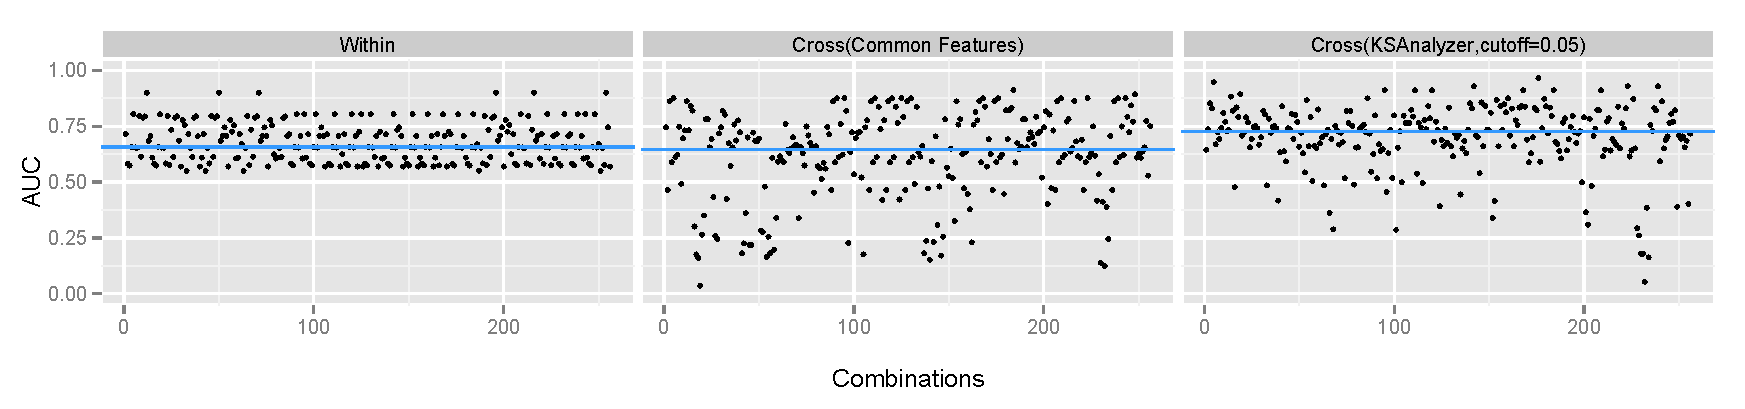
\includegraphics[width=\linewidth]{Figures/Result/auc_compare.pdf}
% 	\caption{Prediction performance comparison among within-results, cross-results
% 	by ASAnalyzer, random analyzer, and manual matching in terms of median AUC values.}
% 	\label{fig:compare_results_on_defect}
% \end{figure*}
% 
% In addition, the median AUC value of all predictions using all defect source
% groups (Defect All in Table~\ref{tab:compare}) is
% 0.701, which is a promising result since the median AUC values in
% within-predictions and cross-predictions by random analyzer and manual matching
% are 0.676, 0.599, and 0.609, respectively. In the case of AEEEM, the median AUC
% of manual feature matching is fairly high (0.673). However, the median AUC of
% within-prediction (0.675) outperforms that of manual feature matching with
% statistical significance (p=0.000).
% 
% Figure~\ref{fig:compare_results_on_defect} shows how each prediction performance
% of within- and cross-predictions varies. The solid line in
% Figure~\ref{fig:compare_results_on_defect} represents the overall prediction
% performance and the mean of all the median AUC values of the targets. Comparing
% the cross-results of AS to within-prediction results, we observed the
% cross-result is better than the within-result. We also compare cross-prediction
% results of AS, random analyzer, and manual matching as well. As we observe, the
% cross-result of AS outperforms that of both random analyzer and manual matching.
% 
% We conducted t-test (p<0.05) for those overall median AUC values between
% within-predictions and cross-predictions of AS. The cross-result of
% AS outperforms the within-result with statistical significance (p=0.002)
% and outperforms those of random analyzer and manual feature matching (p=0.000).
% Thus, we can confirm RQ2; cross-predictions by ASAnalyzer with the cutoff of
% 0.9 outperform to within-predictions in terms of median AUC in our
% experimental setting.


%\begin{result}
%Therefore, we can
%conclude that our cross-domain prediction model can predict defects in targets
%with high coverage
%\end{result}

%--------------------------------------------------------------
% \subsection{Within vs. Cross in non-defect$\Rightarrow$defect}
%--------------------------------------------------------------

% \begin{table}[t]
% \small
% \centering
% \caption{Average AUCs of Within and Cross-prediction results ASAnalyzer with
% Filters and Random Analyzer) by each
% source group in non-defect$\Rightarrow$defect.}
% \label{tab:compare_non_defect}
% \begin{tabular}{|c|c|c|c|c|}
% \hline
% 
% \multirow{2}{*}{\specialcell{{\bf Source}\\{\bf group}}}	&
% \multirow{2}{*}{{\bf Within}}	& \multicolumn{2}{c|}{{\bf Cross}}	&
% \multirow{2}{*}{\specialcell{{\bf Target}\\{\bf coverage}}}
% \\
% 
% \cline{3-4}
% 		& 	& \specialcell{{\bf ASw/F}} & {\bf Random} & \\ \hline
% 
% Effort & 0.63	& 0.84 & 0.73	& 11\% (3/28)\\ \hline
% Severity & N/A  & N/A	& N/A	& 0\% (0/28)\\ \hline
% {\bf SE all}  & {\bf0.63}	& {\bf 0.84} & {\bf 0.73}		& {\bf 11\%} (3/28)\\
% \hline \hline \hline
% Medical	& 0.69	& 0.71	& 0.58	& 32\% (9/28)\\ \hline
% Wine	& 0.57	& 0.55	& 0.57	& 4\% (1/28)\\ \hline \hline
% {\bf non-SE All} & {\bf 0.68}	& {\bf 0.70} & {\bf 0.58}	& {\bf 36\%} (10/28)\\
% \hline
% 
% %{\bf Non-defect All} &{\bf 0.67}	&{\bf 0.73}	&{\bf 0.61} &  \\ \hline
% \end{tabular}
% \end{table}

% Table~\ref{tab:compare_non_defect} shows cross-prediction results in
% non-defect$\Rightarrow$defect in terms of average AUC by each source group.
% Cross-results outperform within-results in non-defect$\Rightarrow$defect as
% well. We conducted the paired t-test for predictions in
% non-defect$\Rightarrow$defect. From the paired t-test, we could conclude that
% cross-results of ASAnalyzer with Filters were comparable to within-results.
% However, we observed very low prediction coverage; 3\% by SE and
% 36\% by non-SE. Thus, we may not generalize this observation, (In
% Section~\ref{sec:prediction_coverage}, we discuss prediction coverage in detail.)
% 
% Random analyzer in Effort in
% Table~\ref{tab:compare_non_defect} outperforms within-predictions in terms of
% average AUC. Note that its within-result is fairly low (0.63). In addition,
% Random analyzer result did not outperform the within-result with statistical significance
% (p=0.18).
% 
% 
% \begin{figure}[t]
% 	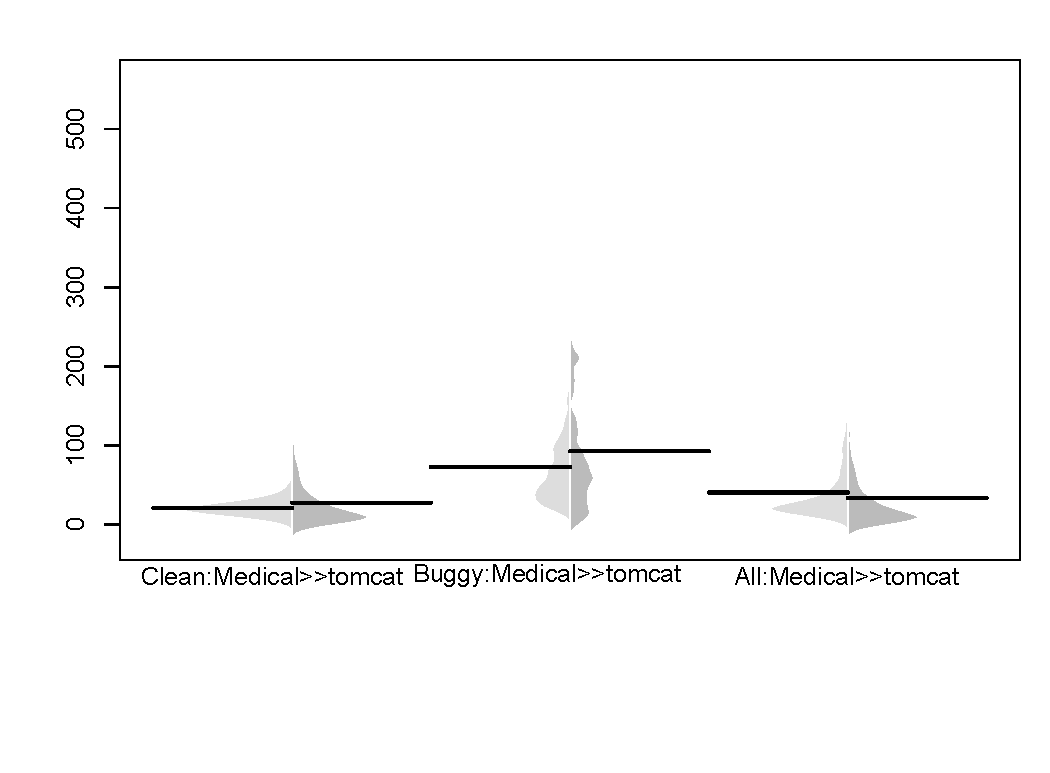
\includegraphics[width=\linewidth]{Figures/Result/medical_dist.pdf}
% 	\caption{Feature distribution of an matched feature from the prediction
% 	combination, Medical(area\_se)$\Rightarrow$Tomcat(rfc), of AUC=0.82.}
% 	\label{fig:medical_dist}
% \end{figure}
% 
% 
% We observed interesting results in Medical. Nine
% out of 28 targets in non-SE$\Rightarrow$defect predictions were covered by
% models from the Medical dataset. An example matched feature is standard error of
% nuclear area of cells (area\_se) of Medical and response for class
% (rfc, to measure coupling) of pc3 in NASA. The area\_se feature represents how
% much irregular the areas of cells are. The higher value of area\_se indicates the higher
% malignancy~\cite{Street93}. This characteristic of the feature, area\_se, is
% similar to that of typical features in defect datasets, as shown in
% Figure~\ref{fig:medical_dist}. We can clearly observe similar distribution
% between the matched features. In addition, original task of the Medical dataset
% was binary classification like software defect prediction in our experimental
% setting. This leads to a bit higher prediction coverage than SE datasets.
% 
% % However, models built by the Wine dataset covered only one target, ar1. This
% % poor coverage of Wine is also due to different characteristics of features from
% % that of typical features used in defect datasets.
% In Wine, ASAnalyzer with Filters is even worse than Random analyzer. In
% addition, models built by the Wine dataset covered only one target.
% Possible explanation is that features in Wine may have different characteristics
% from those in defect datasets and prediction task of Wine is multi-class
% classification rather than binary classification. This may lead
% to different results comparing to that of defect$\Rightarrow$defect.
% 
% For RQ2, we conducted paired t-test for non-defect$\Rightarrow$defect in terms
% of average AUC. Actually, cross-predictions were comparable to
% within-predictions with statistical significant (p=0.15). However, it is hard to
% generalize our result since prediction coverage is very low to conclude RQ2.

% \subsection{Prediction Coverage}
% \label{sec:prediction_coverage}
% 
% % Thus, we could confirm RQ1 in terms of
% % average AUC in our experimental setting. However, we could not confirm RQ3 since
% % prediction coverage of non-defect$\Rightarrow$defect predictions, were too low to compare results.
% 
% 
% \begin{table}[t]
% \small
% \centering
% \caption{Prediction Coverage of ASAnalyzer with Filters (cutoff>0.9) on
% defect$\Rightarrow$defect vs. non-defect$\Rightarrow$defect datasets in terms of
% average AUC.}
% \label{tab:prediction_coverage}
% %\setlength{\tabcolsep}{5pt}
% %\setlength{\extrarowheight}{1.5pt}
% \begin{tabular}{|c|@{ }c@{ }||@{ }c@{ }|@{ }c@{ }|}
% \hline
% \multirow{2}{*}{Target}	& \multirow{2}{*}{defect$\Rightarrow$defect} &
% \multicolumn{2}{c|}{non-defect$\Rightarrow$defect} \\ \cline{3-4}
% & 	& SE$\Rightarrow$defect &
% non-SE$\Rightarrow$defect \\\hline \hline
% EQ			&\cmark	&-&-	\\ \hline
% JDT			&\cmark	&-&\cmark	\\ \hline
% LC			&\cmark	&-&-\\ \hline
% ML			&\cmark	&-&-	\\ \hline
% PDE			&\cmark	&-&-	\\ \hline \hline
% 
% Apache		&\cmark	&-&-	\\ \hline
% Zxing		&\cmark	&-&\cmark	\\ \hline
% Safe		&\cmark	&-&\cmark\\ \hline \hline
% 
% ant-1.3		&\cmark	&-&-	\\ \hline
% arc			&\cmark	&-&-	\\ \hline
% camel-1.0	&\cmark	&-&-	\\ \hline
% poi-1.5		&\cmark	&-&-	\\ \hline
% redaktor	&\cmark	&-&-	\\ \hline
% skarbonka	&\cmark	&-&-	\\ \hline
% tomcat		&\cmark	&- &\cmark	\\ \hline
% velocity-1.4	&\cmark	&-&-	\\ \hline
% xalan-2.4	&\cmark	&-&-	\\ \hline
% xerces-1.2	&\cmark	&-&-	\\ \hline \hline
% 
% cm1			&\cmark	&-&\cmark	\\ \hline
% mw1			&\cmark	&\cmark&\cmark	\\ \hline
% pc1			&\cmark	&-&-	\\ \hline
% pc3			&\cmark	&-&-	\\ \hline
% pc4			&\cmark	&-&\cmark	\\ \hline \hline
% 
% ar1		&\cmark	&-&\cmark	\\ \hline
% ar3		&\cmark	&\cmark&\cmark	\\ \hline
% ar4		&\cmark	&-&\cmark	\\ \hline
% ar5		&\cmark	&\cmark&	\\ \hline
% ar6		&\cmark	&-&-	\\ \hline \hline
% Total & 28/28 (100\%) & 3/28 (11\%) & 10/28 (36\%) \\ \hline

% EQ	&12	&12	\\ \hline
% JDT	&14	&5	\\ \hline
% LC	&12	&11	\\ \hline
% ML	&16	&0	\\ \hline
% PDE	&13	&4	\\ \hline
% 
% Apache	&13	&4	\\ \hline
% Zxing	&20	&18	\\ \hline
% Safe	&17	&12	\\ \hline
% 
% ant-1.3	&9	&9	\\ \hline
% arc	&6	&5	\\ \hline
% camel-1.0	&9	&8	\\ \hline
% poi-1.5	&5	&2	\\ \hline
% redaktor	&10	&0	\\ \hline
% skarbonka	&11	&11	\\ \hline
% tomcat	&6	&4	\\ \hline
% velocity-1.4	&7	&1	\\ \hline
% xalan-2.4	&7	&1	\\ \hline
% xerces-1.2	&9	&0	\\ \hline
% 
% cm1	&17	&16	\\ \hline
% mw1	&9	&9	\\ \hline
% pc1	&14	&4	\\ \hline
% pc3	&12	&1	\\ \hline
% pc4	&15	&0	\\ \hline
% 
% ar1	&15	&15	\\ \hline
% ar3	&17	&16	\\ \hline
% ar4	&16	&16	\\ \hline
% ar5	&14	&12	\\ \hline
% ar6	&11	&10	\\ \hline \hline
% Total & 336 (28) & 206 (24) \\ \hline
% \end{tabular}
% \end{table}

% We checked prediction coverage of our framework for cross-domain defect
% prediction in detail. As shown in Table~\ref{tab:prediction_coverage}, all the
% targets in defect$\Rightarrow$defect could be predicted by our framework. This shows
% prediction coverage of our framework is 100\% in our experimental setting. To
% achieve 100\% coverage, there should exist matched features with high matching
% score ($>$0.9) and the prediction combinations should remain after applying LBM and DM filters. Thus,
% prediction coverage in defect$\Rightarrow$defect clearly shows that features of
% defect datasets could be transferred to build a prediction model and our
% framework could find matched features in defect$\Rightarrow$defect
% predictions.
% 
% However, non-defect$\Rightarrow$defect predictions lead to poor prediction
% coverage. In SE$\Rightarrow$defect prediction, three target projects, mw1, ar3,
% and ar5 are predicted by the framework. This low
% coverage is because of different characteristics of features between defect and
% non-defect datasets. Only three out of all combinations in SE$\Rightarrow$defect
% had co-occurrence features whose matching scores are higher than 0.9. In case
% of the Severity dataset, there were no matched features at all since features of
% the Severity dataset, created by text mining technique such as
% tf*idf~\cite{Menzies08}, are different from typical defect prediction features.


%This poor results in non-defect$\Rightarrow$defect predictions are obvious
% since datasets are collected in too different domains such as severity of
% issue reports and wine quality. We will discuss about this result more,
% particularly, ar5 in SE$\Rightarrow$defect in Section~\ref{sec:Discussion}.
% 
% Somebody may claim the high coverage of defect$\Rightarrow$defect is because of
% many source projects which can make more prediction combinations. In
% non-defect$\Rightarrow$defect predictions, we have few source projects (4)
% comparing to those (15-25) in defect$\Rightarrow$defect predictions for a
% target. However, before applying the HC filter, about 56\% of targets in average
% were already covered by each defect source dataset. This implies that we may
% cover all targets by two or three defect source datasets. In the same setting,
% average prediction coverage by SE and non-SE sources was about 5\% and 18\% respectively.
% 
% In our experimental settings, we could conclude about RQ3:
% \squishlist
% 	\item Our framework for
% cross-domain defect prediction could achieve 100\% prediction coverage in
% defect$\Rightarrow$defect predictions.
% 	\item Non-defect$\Rightarrow$defect predictions are hard to achieve good
% 	prediction coverage since features from different areas are most likely
% 	different from typical features of defect datasets. However, if there exist
% 	datasets whose feature characteristic is similar to that of typical features
% 	from defect datasets and prediction task is similar,i.e. binary classification,
% 	we can increase prediction coverage.
% \squishend
% 
% Due to the low prediction coverage of non-defect$\Rightarrow$defect, we
% only report detailed prediction results of defect$\Rightarrow$defect in
% next sub-sections.


\subsection{Win/Tie/Loss Results}

\begin{table}[!t]
%\small
\scriptsize
\centering
\caption{Win/Tie/Loss results of HDP by KSAnalyzer (cutoff=0.05)
against WPDP (Baseline1), CPDP-CM (Baseline2), and CPDP-IFS (Baseline3).}
\label{tab:win_results}
%\setlength{\tabcolsep}{5pt}
%\setlength{\extrarowheight}{1.5pt}
%\begin{tabular}{|@{ }c@{ }||@{ }c@{ }|@{ }c@{ }|@{ }c@{ }||@{ }c@{ }|@{ }c@{
%}|@{ }c@{ }|}
\begin{tabular}{|@{ }c@{}||@{ }c@{ }|@{ }c@{ }|@{ }c@{}||@{ }c@{ }|@{ }c@{
}|@{ }c@{}||@{ }c@{ }|@{ }c@{ }|@{ }c@{}|}
\hline

\multirow{3}{*}{{\bf Target}}
&\multicolumn{9}{c|}{\bf Against}
\\ \cline{2-10}
&\multicolumn{3}{c||}{\specialcell{{\bf WPDP}\\{(Baseline1)}}}
&\multicolumn{3}{c||}{\specialcell{{\bf CPDP-CM}\\{(Baseline2)}}}
&\multicolumn{3}{c|}{\specialcell{{\bf CPDP-IFS}\\{(Baseline3)}}}
\\
\cline{2-10}

& Win & Tie & Loss & Win & Tie & Loss & Win & Tie & Loss \\ \hline \hline

EQ			&4	&0	&0 & 2 & 2 & 0 &4 &0 &0 	\\ \hline
JDT			&0	&0	&5 & 3 & 0 & 2 &5 &0 &0	\\ \hline
LC			&6	&0	&1 & 3 & 3 & 1 &3 &1 &3	\\ \hline
ML			&0	&0	&6 & 4 & 2 & 0 &6 &0 &0	\\ \hline
PDE			&3	&0	&2 & 2 & 0 & 3 &5 &0 &0	\\ \hline \hline

Apache		&6	&0	&5 & 8 & 1 & 2 &9 &0 &2	\\ \hline
Safe		&14	&0	&3 & 12 & 0 & 5 &15 &0 &2	\\ \hline
Zxing		&8	&0	&0 & 6 & 0 & 2 &7 &0 &1	\\ \hline \hline

ant-1.3		&6	&0	&1 & 6 & 0 & 1 &5 &0 &2 \\ \hline
arc			&3	&1	&0 & 3 & 0 & 1 &4 &0 &0 \\ \hline
camel-1.0	&3	&0	&2 & 3 & 0 & 2 &4 &0 &1 \\ \hline
poi-1.5		&2	&0	&2 & 3 & 0 & 1 &2 &0 &2 \\ \hline
redaktor	&0	&0	&4 & 2 & 0 & 2	&3 &0 &1 \\ \hline
skarbonka	&11	&0	&0 & 4 & 0 & 7 &9 &0 &2 \\ \hline
tomcat		&2	&0	&0 & 1 & 1 & 0 &2 &0 &0 \\ \hline
velocity-1.4	&0	&0	&3 & 0 & 0 & 3 &0 &0 &3 \\ \hline
xalan-2.4	&0	&0	&1 & 1 & 0 & 0 &1 &0 &0	\\ \hline
xerces-1.2	&0	&0	&3 & 3 & 0 & 0 &1 &0 &2	\\ \hline \hline

cm1			&7	&1	&2 & 8 & 0 & 2 &9 &0 &1	\\ \hline
mw1			&5	&0	&1 & 4 & 0 & 2 &4 &0 &2	\\ \hline
pc1			&1	&0	&5 & 5 & 0 & 1 &6 &0 &0	\\ \hline
pc3			&0	&0	&7 & 7 & 0 & 0 &7 &0 &0	\\ \hline
pc4			&0	&0	&7 & 2 & 0 & 5 &7 &0 &0	\\ \hline \hline

ar1		&14	&0	&1	& 14 & 0 & 1 &11 &0 &4 \\ \hline
ar3		&15	&0	&0	& 5 & 0 & 10 &10 &2 &3 \\ \hline
ar4		&16	&0	&0	& 14 & 1 & 1 &15 &0 &1 \\ \hline
ar5		&14	&0	&4	& 14 & 0 & 4 &16 &0 &2 \\ \hline
ar6		&7	&1	&7	& 8 & 4 & 3  &12 &0 &3 \\ \hline \hline
Total & \specialcell{{147}\\{66.2\%}} &\specialcell{{3}\\{1.4\%}}
&\specialcell{{72}\\{32.4\%}}
& \specialcell{{147}\\{66.2\%}} &\specialcell{{14}\\{6.3\%}}
&\specialcell{{61}\\{27.5\%}}
& \specialcell{{182}\\{82.0\%}} &\specialcell{{3}\\{1.3\%}}
&\specialcell{{37}\\{16.7\%}}
\\
\hline
\end{tabular}
\end{table}


To investigate our performance evaluation in detail, we report
the Win/Tie/Loss results of HDP by KSAnalyzer with the cutoff of 0.05 against
WPDP (Baseline1), CPDP-CM (Baseline2), and CPDP-IFS
(Baseline3) in Table~\ref{tab:win_results}.


KSAnalyzer with the cutoff of 0.05 conducted 222 out of 600 prediction
combinations since 378 combinations do not have any matched
metrics because of the cutoff threshold. In
Table~\ref{tab:win_results}, the target dataset, EQ, was predicted in four
prediction combinations and our approach, HDP, outperforms Baseline1 and
Baseline3 in the four combinations (i.e. 4 Wins). However, HDP outperforms
Baseline2 in only two combinations of the target, EQ (2 Wins). 


% \subsection{Matched features}
% In this section, we discuss matched features to investigate prediction
% performance on cross-domain defect prediction in detail.

% A reason why ASAnalyzer can predict defects pretty well on cross-domain
% settings is that most defect prediction metrics usually represent complexity of
% source code and its change; it tends to be more buggy when the complexity is
% higher.
Against Baseline1, the six targets such as EQ, Zxing, skarbonka, tomcat,
ar3, and ar4 have only Win results. In other words, defects in those six targets
could be predicted better by other source projects using HDP models by
KSAnalyzer compared to WPDP models.

However, the eight targets such as JDT, ML, redaktor, velocity-1.4, xalan-2.4,
xerces-1.2, pc3, and pc4 have no Wins at all against Baseline1. In
addition, other targets still have Losses even though they have Win or Tie
results.

Overall, the numbers of Win and
Tie results are 147 and 3 respectively out of all of the 222 prediction
combinations.
This means that about 67.6\% of prediction combinations by our HDP
models achieve better or comparable prediction performance than those in
WPDP.

The Win/Tie/Loss results against Baseline2 and Baseline3 show a similar trend.
The HDP results in the 161 (72.5\%) out of 222 prediction combinations show
HDP outperforms and is comparable to CPDP-CM. Against Baseline3, 185
(83.3\%) predction combinations are Win or Tie results.

The Win/Tie/Loss results show that with our HDP model by
KSAnalyzer there is a higher possibility of getting a better prediction
performance.

However, there are still about 32\% Loss results against WPDP. In
Section~\ref{sec:Discussion}, we discuss and analyze why Loss results happen.


% In the SOFTLAB group, all projects get Win results
% which represent that average AUC of cross-prediction results outperform
% within-prediction results with statistical significance (the paired t-test,
% p=0.05).
% 
% There is one Tie result in cm1 of the NASA group. The Tie represents that
% a cross-prediction result is comparable to a within-prediction result with
% statistical significance. Overall, Win (17) and Tie (1) results are 18 out of 28
% predictions. Comparing to Loss results, many cross-predictions (64\%) have
% better or comparable results to within-predictions. In terms of Loss
% results, 10 predictions did not outperform within-results. 
%Even though some
% predictions have Loss results, their within-prediction results are already high
% and cross-prediction results are also pretty good, i.e. pc3 (0.76) and pc4(0.76) in NASA.
% In Section~\ref{sec:Discussion}, we will discuss why some predictions got Loss
% results in detail.

% \begin{table}[t]
% \small
% \centering
% \caption{Win/Tie/Loss results of cross-predictions against within-predictions
% in terms of average AUC.}
% \label{tab:win_results}
% %\setlength{\tabcolsep}{5pt}
% %\setlength{\extrarowheight}{1.5pt}
% \begin{tabular}{|@{ }c@{ }|@{ }c@{ }|@{ }c@{ }|@{ }c@{ }|@{ }c@{ }|}
% \hline
% Group 	& Target	& Within AUC	& Cross AUC & Result \\\hline
% \hline
% \multirow{4}{*}{AEEEM} & EQ			& 0.58	& 0.77	& Win	\\ \cline{2-5}
% & JDT			& 0.79	& 0.82	& Win	\\ \cline{2-5}
% & LC			& 0.57	& 0.79	& Win	\\ \cline{2-5}
% & ML			& 0.73	& 0.53	& Loss	\\ \cline{2-5}
% & PDE			& 0.68	& 0.67	& Loss	\\ \hline \hline
% 
% \multirow{3}{*}{ReLink} &Apache		& 0.71	& 0.68 	& Loss	\\ \cline{2-5}
% & Zxing		& 0.60	& 0.62	& Win	\\ \cline{2-5}
% & Safe		& 0.70	& 0.87	& Win	\\ \hline \hline
% 
% \multirow{10}{*}{MORPH} &ant-1.3		& 0.61	& 0.83	& Win	\\ \cline{2-5}
% & arc			& 0.66	& 0.79	& Win	\\ \cline{2-5}
% & camel-1.0	& 0.53	& 0.64	& Win	\\ \cline{2-5}
% & poi-1.5		& 0.70	& 0.73 	& Win	\\ \cline{2-5}
% & redaktor	& 0.74	& 0.45	& Loss	\\ \cline{2-5}
% & skarbonka	& 0.56	& 0.73	& Win	\\ \cline{2-5}
% & tomcat		& 0.78	& 0.79 	& Win	\\ \cline{2-5}
% & velocity-1.4	& 0.72	& 0.56	& Loss	\\ \cline{2-5}
% & xalan-2.4	& 0.75	& 0.68	& Loss	\\ \cline{2-5}
% & xerces-1.2	& 0.62	& 0.55	& Loss	\\ \hline \hline
% 
% \multirow{5}{*}{NASA} &cm1			& 0.63	& 0.64	& Tie	\\ \cline{2-5}
% & mw1			& 0.60	& 0.72	& Win	\\ \cline{2-5}
% & pc1			& 0.78	& 0.68	& Loss	\\ \cline{2-5}
% & pc3			& 0.79	& 0.76	& Loss	\\ \cline{2-5}
% & pc4			& 0.9	& 0.76	& Loss	\\ \hline \hline
% 
% \multirow{5}{*}{SOFTLAB} & ar1			& 0.57	& 0.73	& Win	\\ \cline{2-5}
% & ar3			& 0.55	& 0.84	& Win	\\ \cline{2-5}
% & ar4			& 0.64	& 0.82	& Win	\\ \cline{2-5}
% & ar5			& 0.75	& 0.93	& Win	\\ \cline{2-5}
% & ar6			& 0.64	& 0.74	& Win	\\ \hline \hline
% \multicolumn{5}{c}{Win: 17, Tie: 1, Loss: 10} \\ \hline
